\documentclass[11pt]{article}
\usepackage[utf8]{inputenc}
\usepackage[pdftex]{graphicx}
\usepackage{pdfpages}
\usepackage[english]{babel}
\usepackage [autostyle, english = american]{csquotes}
\usepackage{mathtools}
\usepackage{float}
\usepackage{xcolor}
\usepackage{listings}
\usepackage{fancyvrb}
\usepackage{caption,subcaption}
%\usepackage{subfigure}
\usepackage[margin=0.6in]{geometry}
\usepackage{adjustbox}
\usepackage{listings}
\usepackage{hyperref}
\usepackage{wrapfig}
\usepackage{newfloat}
\usepackage[cm]{fullpage}
\usepackage[cachedir=build,newfloat,outputdir=build]{minted}
\usepackage{verbatim}

\definecolor{mintedbackground}{rgb}{0,0,0}
\usemintedstyle{tango}
\newenvironment{code}{\captionsetup{type=listing}}{}
\SetupFloatingEnvironment{listing}{name=Source Code}
\captionsetup[subfigure]{subrefformat=simple,labelformat=simple}
\renewcommand{\thelisting}{\arabic{listing}}
\renewcommand\thesubfigure{(\alph{subfigure})}
\definecolor{lightgray}{rgb}{.7,.7,.7}
\definecolor{gray}{rgb}{.4,.4,.4}
\definecolor{darkblue}{rgb}{0,0,.3}
\definecolor{gray}{rgb}{0.4,0.4,0.4}
\definecolor{darkblue}{rgb}{0.0,0.0,0.6}
\definecolor{cyan}{rgb}{0.0,0.6,0.6}
\renewcommand{\thelisting}{\arabic{listing}}
\renewcommand\thesubfigure{(\alph{subfigure})}

\definecolor{termback}{HTML}{DBE0E0}
\definecolor{termkeyword}{HTML}{50DA8B}
\lstdefinestyle{Bash}
{language=bash,
keywordstyle=\color{termkeyword},
basicstyle=\ttfamily,
morekeywords={@.},
alsoletter={:~\$.},
morekeywords=[2]{peter@kbpet:},
keywordstyle=[2]{\color{termkeyword}},
literate={\$}{{\textcolor{termkeyword}{\$}}}1 
         {:}{{\textcolor{termkeyword}{:}}}1
         {~}{{\textcolor{termkeyword}{\textasciitilde}}}1,
}

\geometry{
 a4paper,
 total={170mm,257mm},
 left=10mm,
 right=10mm,
 top=10mm,
 bottom=15mm
}
\graphicspath{ {images/} }

\lstset{
  basicstyle=\ttfamily,
  columns=fullflexible,
  showstringspaces=false,
  commentstyle=\color{gray}\upshape
}

\hypersetup{
    colorlinks,
    citecolor=black,
    filecolor=black,
    linkcolor=black,
    urlcolor=blue
}
 \newmintedfile[pycode]{python3}{
frame=lines,
framesep=2mm,
fontsize=\footnotesize,
showtabs =false,
autogobble=true,
breaklines=true,
mathescape=true
}
 \newmintedfile[shellcode]{bash}{
frame=lines,
framesep=2mm,
fontsize=\footnotesize,
showtabs =false,
autogobble=true,
breaklines=true,
mathescape=true
}

\newmintedfile[rcode]{S}{
frame=lines,
framesep=2mm,
fontsize=\footnotesize,
showtabs =false,
autogobble=true,
breaklines=true,
mathescape=true
}
\newmintinline[ibash]{bash} {
}

\newmintinline[ipy]{python3} {
}
\RecustomVerbatimCommand{\VerbatimInput}{VerbatimInput}%
{fontsize=\footnotesize,
 %
 frame=lines,  % top and bottom rule only
 framesep=2em, % separation between frame and text
 %
 labelposition=topline,
 %
 commandchars=\|\(\), % escape character and argument delimiters for
                      % commands within the verbatim
 commentchar=*        % comment character
}

\newcommand*{\escape}[1]{\texttt{\textbackslash#1}}

\title{Assignment 4 \\ Introduction to Information Retrieval \\ CS734/834}
\author{John Berlin}
\date{\today}
\renewcommand\thesection{Q.\arabic{section}}
\renewcommand\thesubsection{\thesection}
\begin{document}
\maketitle
\newpage
\section*{Note}

\indent During the course of this class I have found myself having to reusing code from previous assignments and re-working them for use in the current question I am working on at the time. This came to a head in this assignment where the changes to existing code became non-trivial which lead me to create more generalized versions of common operations used throughout this course. In order to keep the answers to questions about the methodology used in answering rather than implementation details using these generalized methods I will explain what they do here. The python3 classes seen in \autoref{code:cntx} are to be utilized with the context control statement \ipy{with} most commonly used with the \ipy{open} statement which opens a file object and automatically closes it when the control flow of the program exits that context. This is en-essence what each of these classes do. \newline   \newline  

The BeautifulSoupFromFile classes takes the path to a file plus the parser type used when creating the soup i.e html or xml and returns to the context using it the soup produced from opening the file and creating a new BeautifulSoup. AutoSaver and AutoSaveCsv takes the type to be save (python list or dictionary) with the path to the file to be written and returns to the calling context an empty version of the type specified to be populated in the scope of that context finally saving the types content to the file path when the context is exited. They also take optional arguments of functions which are used to format the output and or select what entities in they save type to be written to file. RunCommandSaveOut classes takes a function producing a \ipy{subprocess.Popopen} class, the command line arguments to pass to the function and supplies the function with a file object by which the standard output of the spawned process is serialized to. CleanFileLines class reads the contents of a specified file and applies a cleaning function to the contents (for example: $f(``A,B,C,X,Y,Z\escape{n}") \to ``A,B,C"$ ) returning to the context the cleaned lines with the option to save the cleaned lines back to the originating file. FileLinePrinter operates similarly but only prints the raw lines of the specified files. SelectFromFile also applies a transformation function to the files content but also applies a selector function to the cleaned contents of the file returning to the context only what is produced  after applying it to the files contents. RandFinderFile operates similarly but the selection function supplied is to randomly select a line from the files content which is then returned to the context.  \newline   \newline  

The other functions used in answering the questions in this assignment follow the convention of the previous assignments defining less intensive helpers in the file util.py seen in \autoref{code:util}.  Also the shell script created to run galago commands in assignment 3 \autoref{code:rungal} was also utilized with the eval argument which sets up the correct command line arguments to run the galago function eval as the  default options for this do not return results required for this assignment. A more specialized utility file was created for use with the context classes described previously for use with the output of galago functions especially for sanatizing the output of the query runs to work with the eval function of galago. These functions can be seen in \autoref{code:cacm_help}.  \newline \newline Finally it must also be noted that I will be using an updated version of galago (v3.10) in this report. For a more detailed explanation as to why and the differences in this version from the one used by the textbook please consult this same section in the report for assignment 3 for more details.
\newpage
\section{Question 8.3} \label{q1}
\begin{verbatim}
For one query in the CACM collection (provided at the book website), 
generate a ranking using Galago, and then calculate average precision, NDCG at 5
and 10, precision at 10, and the reciprocal rank by hand.
\end{verbatim}
\subsection{Answer} 
Like the previous assignments questions where galago was used to query a collection creation of the index and query creation is the first step. This process was automated thanks to the lessons learned from having used galago before and having the queries were supplied to us. Since the provided queries are in the old xml style they are converted to json after the index has been created.  The automation process can be seen in the python file \textbf{q1\_cacm\_query\_rel.py}, \autoref{code:q1} along with the rest of the code used in answering this question. Running the file \ibash{python3 q1_cacm_query_rel.py} for the first time will create the index, convert the queries and after the running the queries against the CACM collection execute the \textit{eval} function of galago against the runs results automatically. Subsequent executions of this file will not run the galago commands if the files produced by running this file are found to exist. The first time output generated can be seen in  \autoref{fig:cacmidx}.
\begin{figure}[H]
\centering
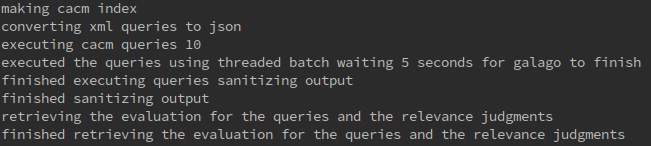
\includegraphics[scale=0.7]{q1buildidx.png}
\caption{Building CACM collection index}
\label{fig:cacmidx}
\end{figure}
Their is an extra step noted in the output generated by this python, \autoref{fig:cacmidx}, which is \textit{finished executing queries sanitizing output}. This extra step is required in order for the eval function of galago to work properly. The batch search function of galago as stated in the \href{https://sourceforge.net/p/lemur/wiki/Galago\%20Functions/}{documentation} produces output in the following format 
\begin{verbatim}
<qid> Q0 <docid> <rank> <score> <system-name> <begin> <end>
\end{verbatim}
Running the batch search command made the \textit{docid} part of the output contain the full path to a CACM document on my machine. The full path for the docid caused the \textbf{eval} function of galago to not produce any output. This puzzled me for upwards of thirty minutes as I attempted to figure out why by recreating the index and playing around with various parameters to the \textbf{batch-search} function. It was not until I looked at the provided \textit{cacm.rel} file provided on the textbooks webcite. \autoref{fig:cacmrel} shows the first few lines of this file.
\begin{figure}[H]
\centering
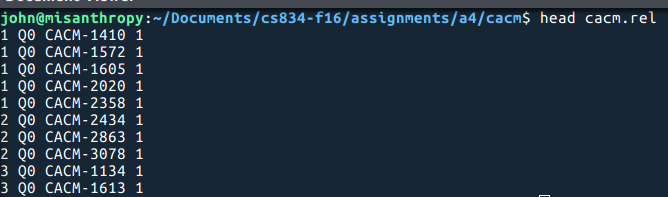
\includegraphics[scale=0.8]{camrell.png}
\caption{head cacm.rel}
\label{fig:cacmrel}
\end{figure}
As you can see in the output of running the unix command \textit{head} on the file there is only the name of the file contained in the collection with the query number it is relevant for and a weight (Q0 is disregarded by galago). On inspection I realized that galago must not be able to match a queries returned documents to the relevance file if they contain the full path to them. I could not find any option to suppress this in the output for the runs so cleaning the runs results to be in the form $<quid \ Q0 \ docid \ rank \ score>$  in order to be matched with the relevance file was the only way forward. After sanitizing the output the the relevance results for the run can was determined. Now the question stated \textbf{the reciprocal rank by hand} after a list of metrics to be calculated which could mean just the reciprocal rank or all of them but it also can be roughly coerced into the interpretation of by code utilizing values produced by code you wrote which is how I interpreted its meaning.  Plus I wanted to use a python file I found on gist a while back ;) which can be seen in \autoref{code:q1rnk}. \newline \newline
The query for the metrics calculation is selected by random from the runs results and then calculated by hand written code along with the output of the same metrics as galago computed them for a sanity check. The by hand calculation is done as following: select a random run from the batch-search runs \textit{eval} results output, select the relevant documents for that run from the \textit{cam.rel} file and  then select that runs returned documents from the batch-search output. If the run had relevant documents or the \textit{eval} results for query did not have NaN computed by galago for the metrics do the by hand computation of the metrics.  Queries 34 35 41 46 47 50 51 52 53 54 55 56 had NaN values for the metrics when calculated by galago\newline \newline
For each document returned by the query create a list of binary values indicated if the returned document at position $n$ was relevant (1) or not (0) then calculate NDCG@5 and NDCG@10, P@10, Average Precision using the created list plus the Reciprocal Rank. This process was done for three randomly chosen query 4 \autoref{fig:cam_rel4}, query 9 \autoref{fig:cam_rel9} and query 11 \autoref{fig:cam_rel11}, along with the galago computed scores for NDCG@5 and NDCG@10, P@10. It must be noted that galago computes Average Precision for MAP when consulting the source code to discover the available metrics. As seen in the figures the computed P@10 values for all three queries match the calculation done by galago while the NDCG values for queries 4 and 9 are way off in comparison to galago computed versions whereas query 11 had computed NDCG values off by only $.01$ for NDCG@5 and $.17$ for NDCG@10. Consulting the methods used to compute these metrics besides using numpy to calculate the score the methods for all intents and purposes are implemented correctly.  The number of returned documents for each each query was set to ten when executed using galago as the Google only 10 results per page in its search results.  As seen in the output queries 4,9 and 11 have 12, 9, and 19 relevant  documents respectfully according to the provided \textit{cam.rel} used in answering this question. This leads me to believe that galago is considering the full set of relevant documents in the calculations it returns. 
\begin{figure}[H]
\centering
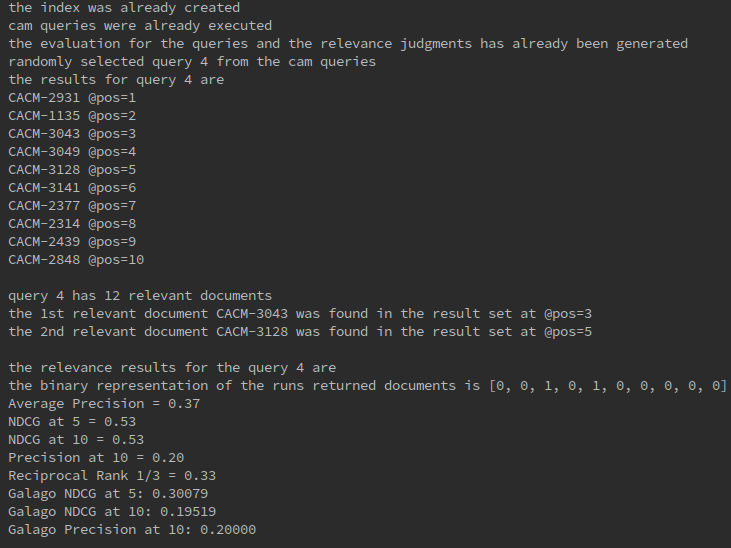
\includegraphics[scale=0.6]{q1run2.png}
\caption{Relevance Metrics For Queries 4}
\label{fig:cam_rel4}
\end{figure}

\begin{figure}[H]
\centering
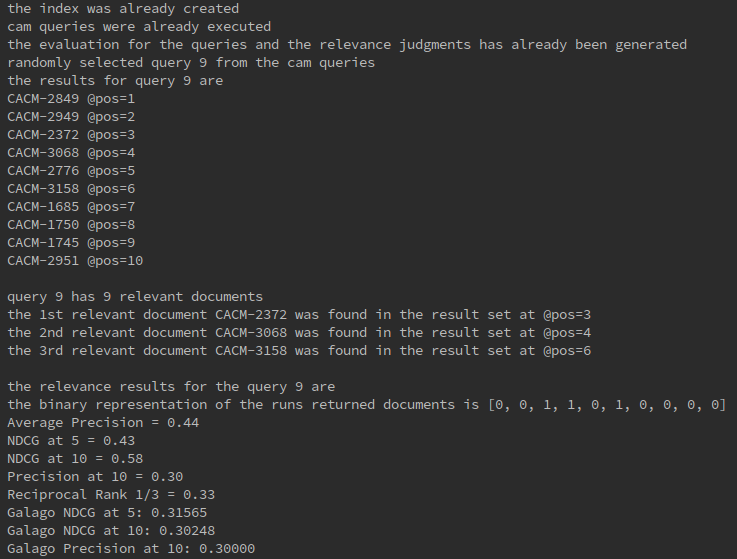
\includegraphics[scale=0.6]{q1_run3.png}
\caption{Relevance Metrics For Query 9}
\label{fig:cam_rel9}
\end{figure}
\begin{figure}[H]
\centering
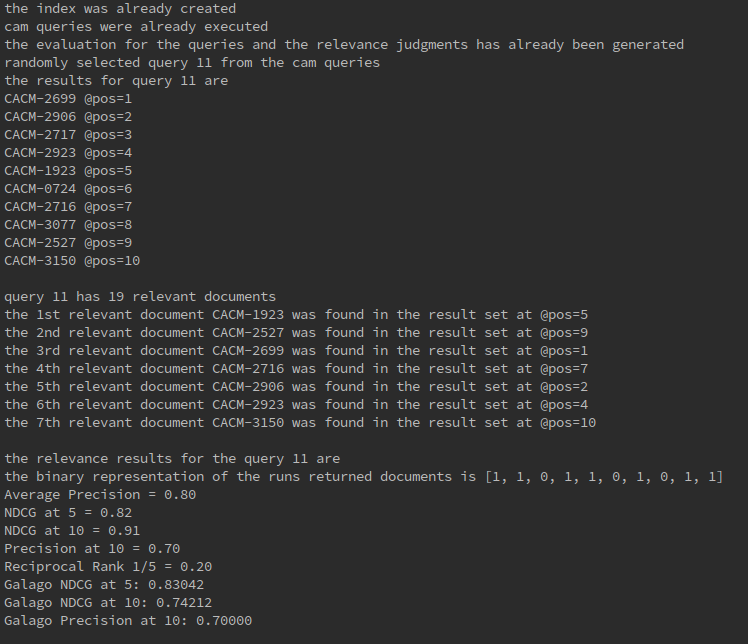
\includegraphics[scale=0.6]{q1run1.png}
\caption{Relevance Metrics For Query 11}
\label{fig:cam_rel11}
\end{figure}
\begin{code}
\captionof{listing}{Single CACM Query Relevance} 
\label{code:q1}
	\pycode{code/q1_cacm_query_rel.py}
\end{code}
\newpage
\section{Question 8.5} \label{q2}
\begin{verbatim}
Generate the mean average precision, recall-precision graph, average NDCG
at 5 and 10, and precision at 10 for the entire CACM query set
\end{verbatim}
\subsection{Answer} 
The values used in the graph for this question were retrieved from the results generated from \textit{eval} function used in \autoref{q1} and then saved to a csv file \autoref{code:q2py} for plotting via R \autoref{code:q2r}. It must be noted that the R-Precision (color red) was not asked for by this question but was included as the R values corresponds to the number of returned documents for a query. This was to done in attempt to confirm my suspicions about how galago computes the internally as noted in \autoref{q1}. and to provide an baseline by which the other metrics can be compared to.
 \autoref{fig:q2plot} shows the metrics plotted against each and it is clear to see that results follow a similar pattern.
\begin{figure}[H]
\centering
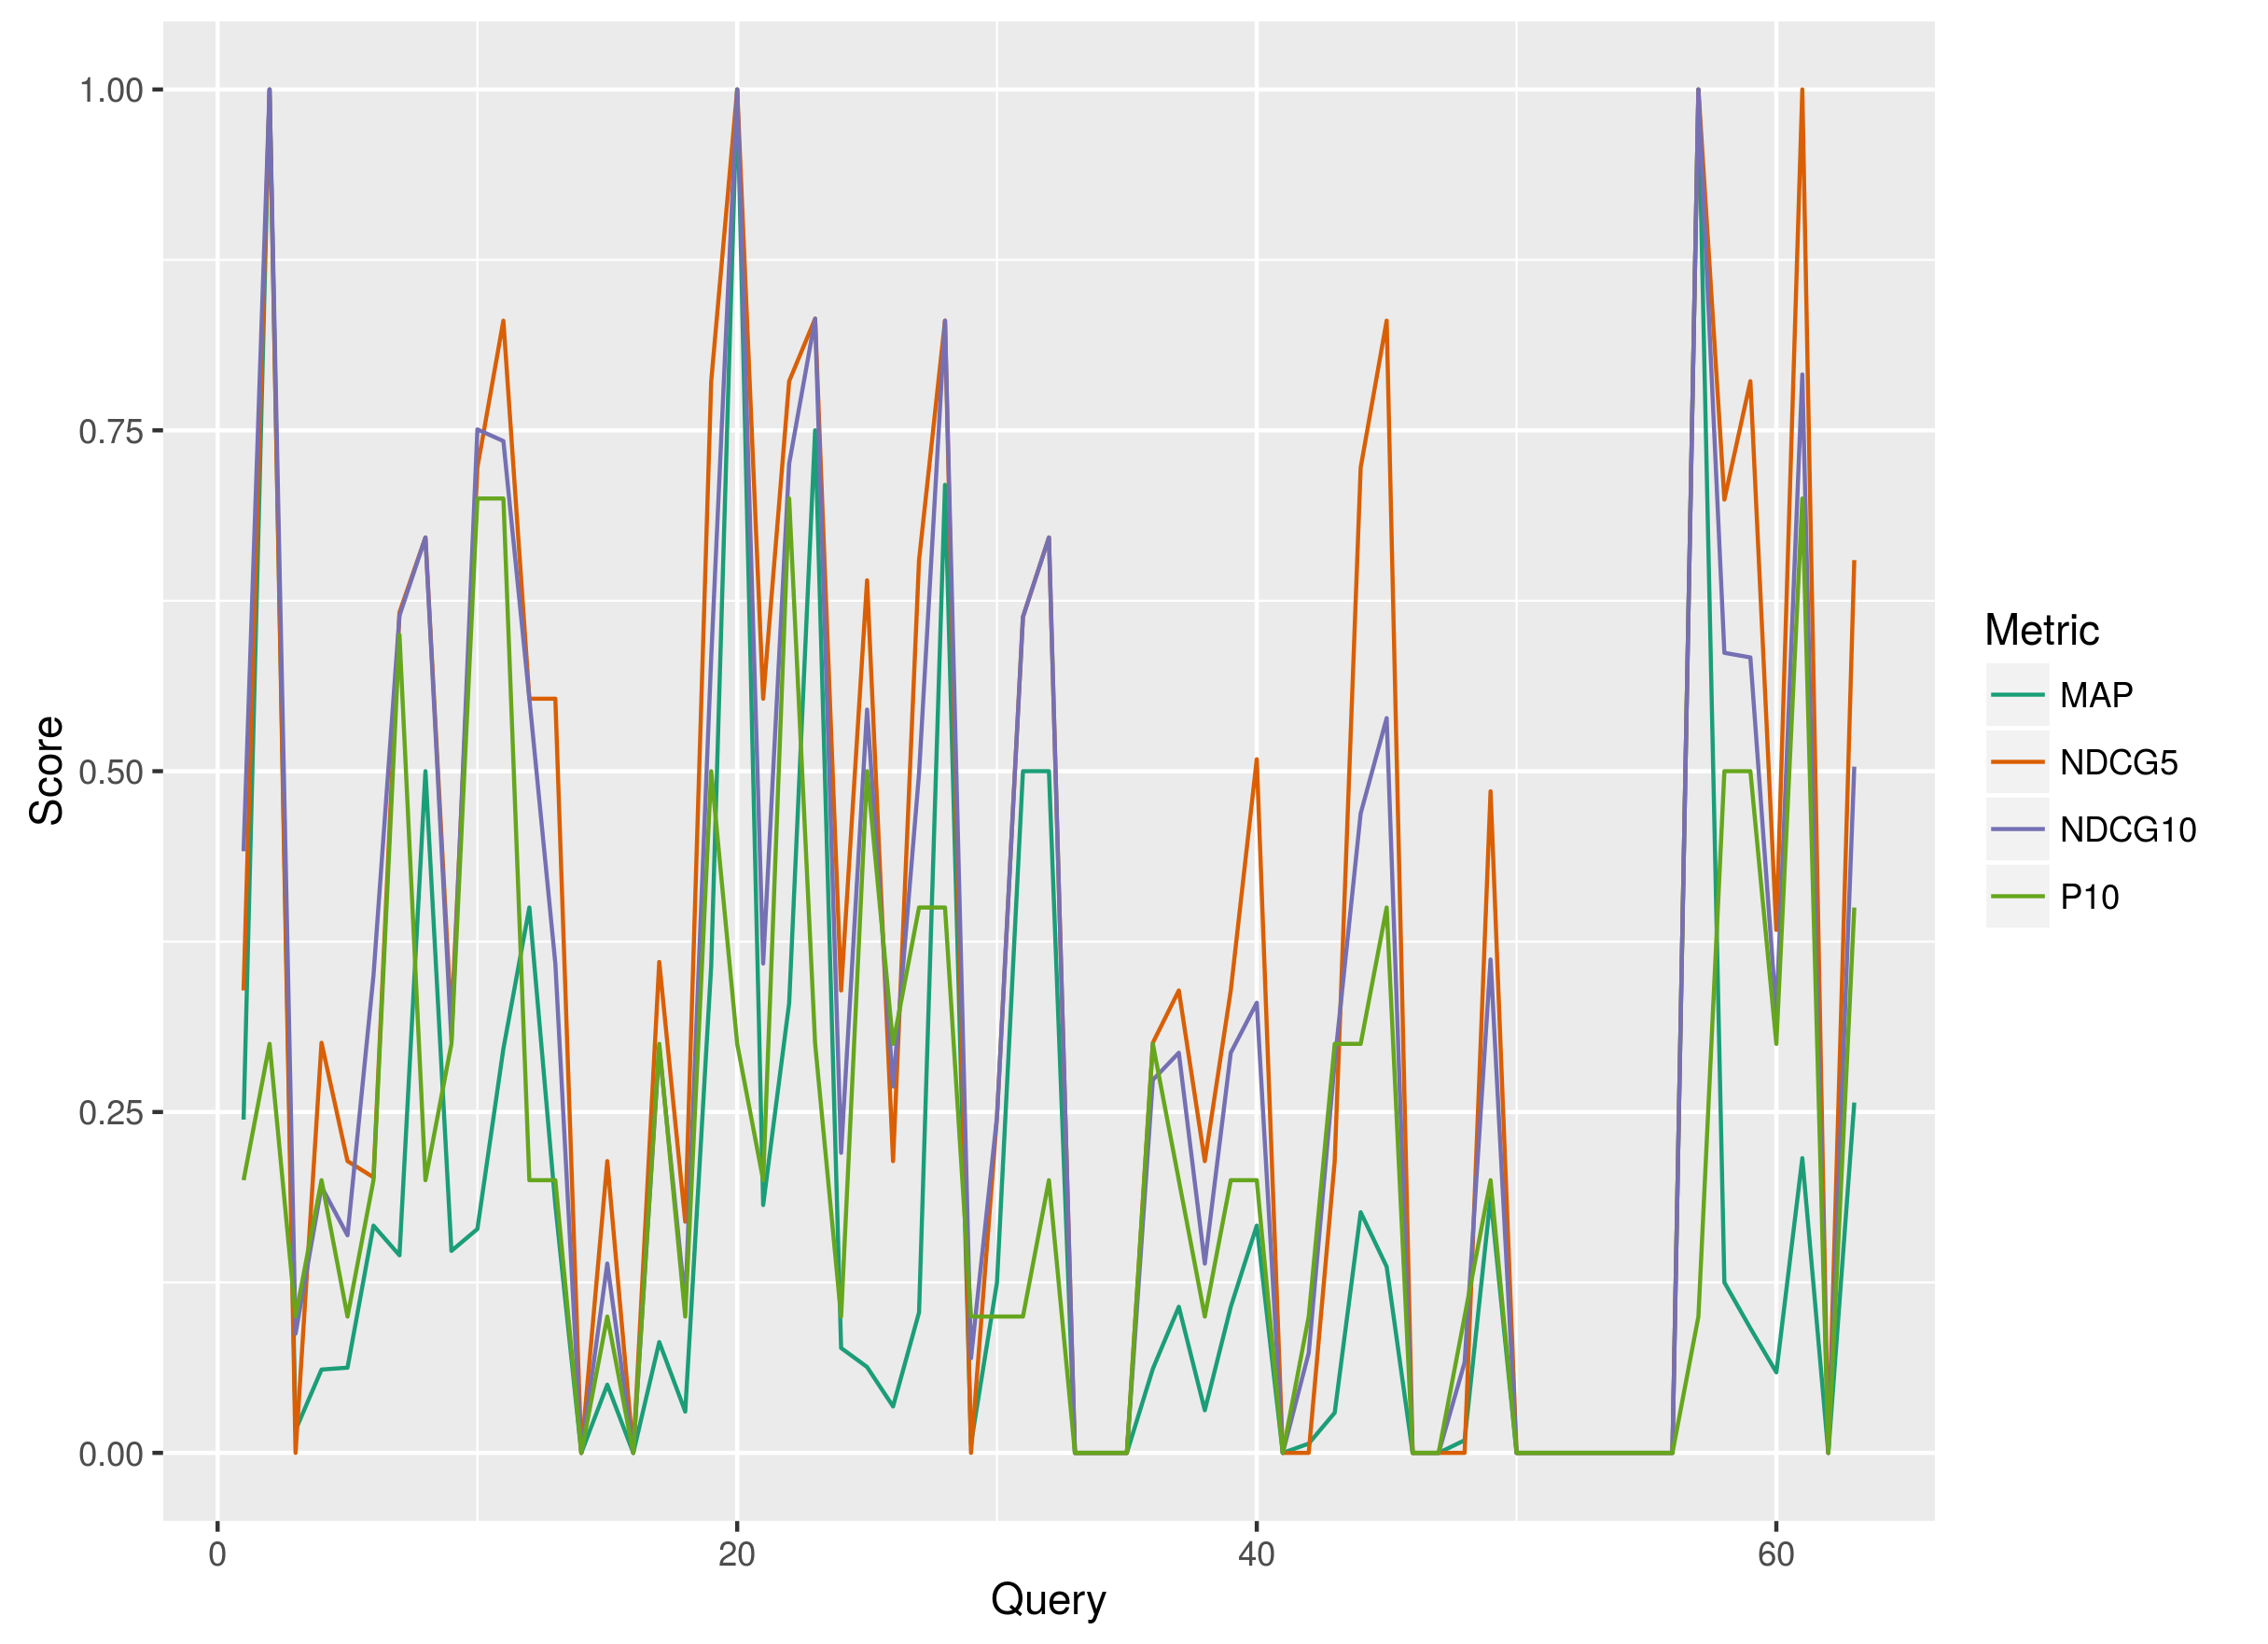
\includegraphics[scale=0.9]{q2_plot.png}
\caption{Galago Eval Metrics For All Queries}
\label{fig:q2plot}
\end{figure}
This is also evident when considering \autoref{fig:q2plot2} which plots the Recall and Precision scores for each query as calculated by galago. 
\begin{figure}[H]
\centering
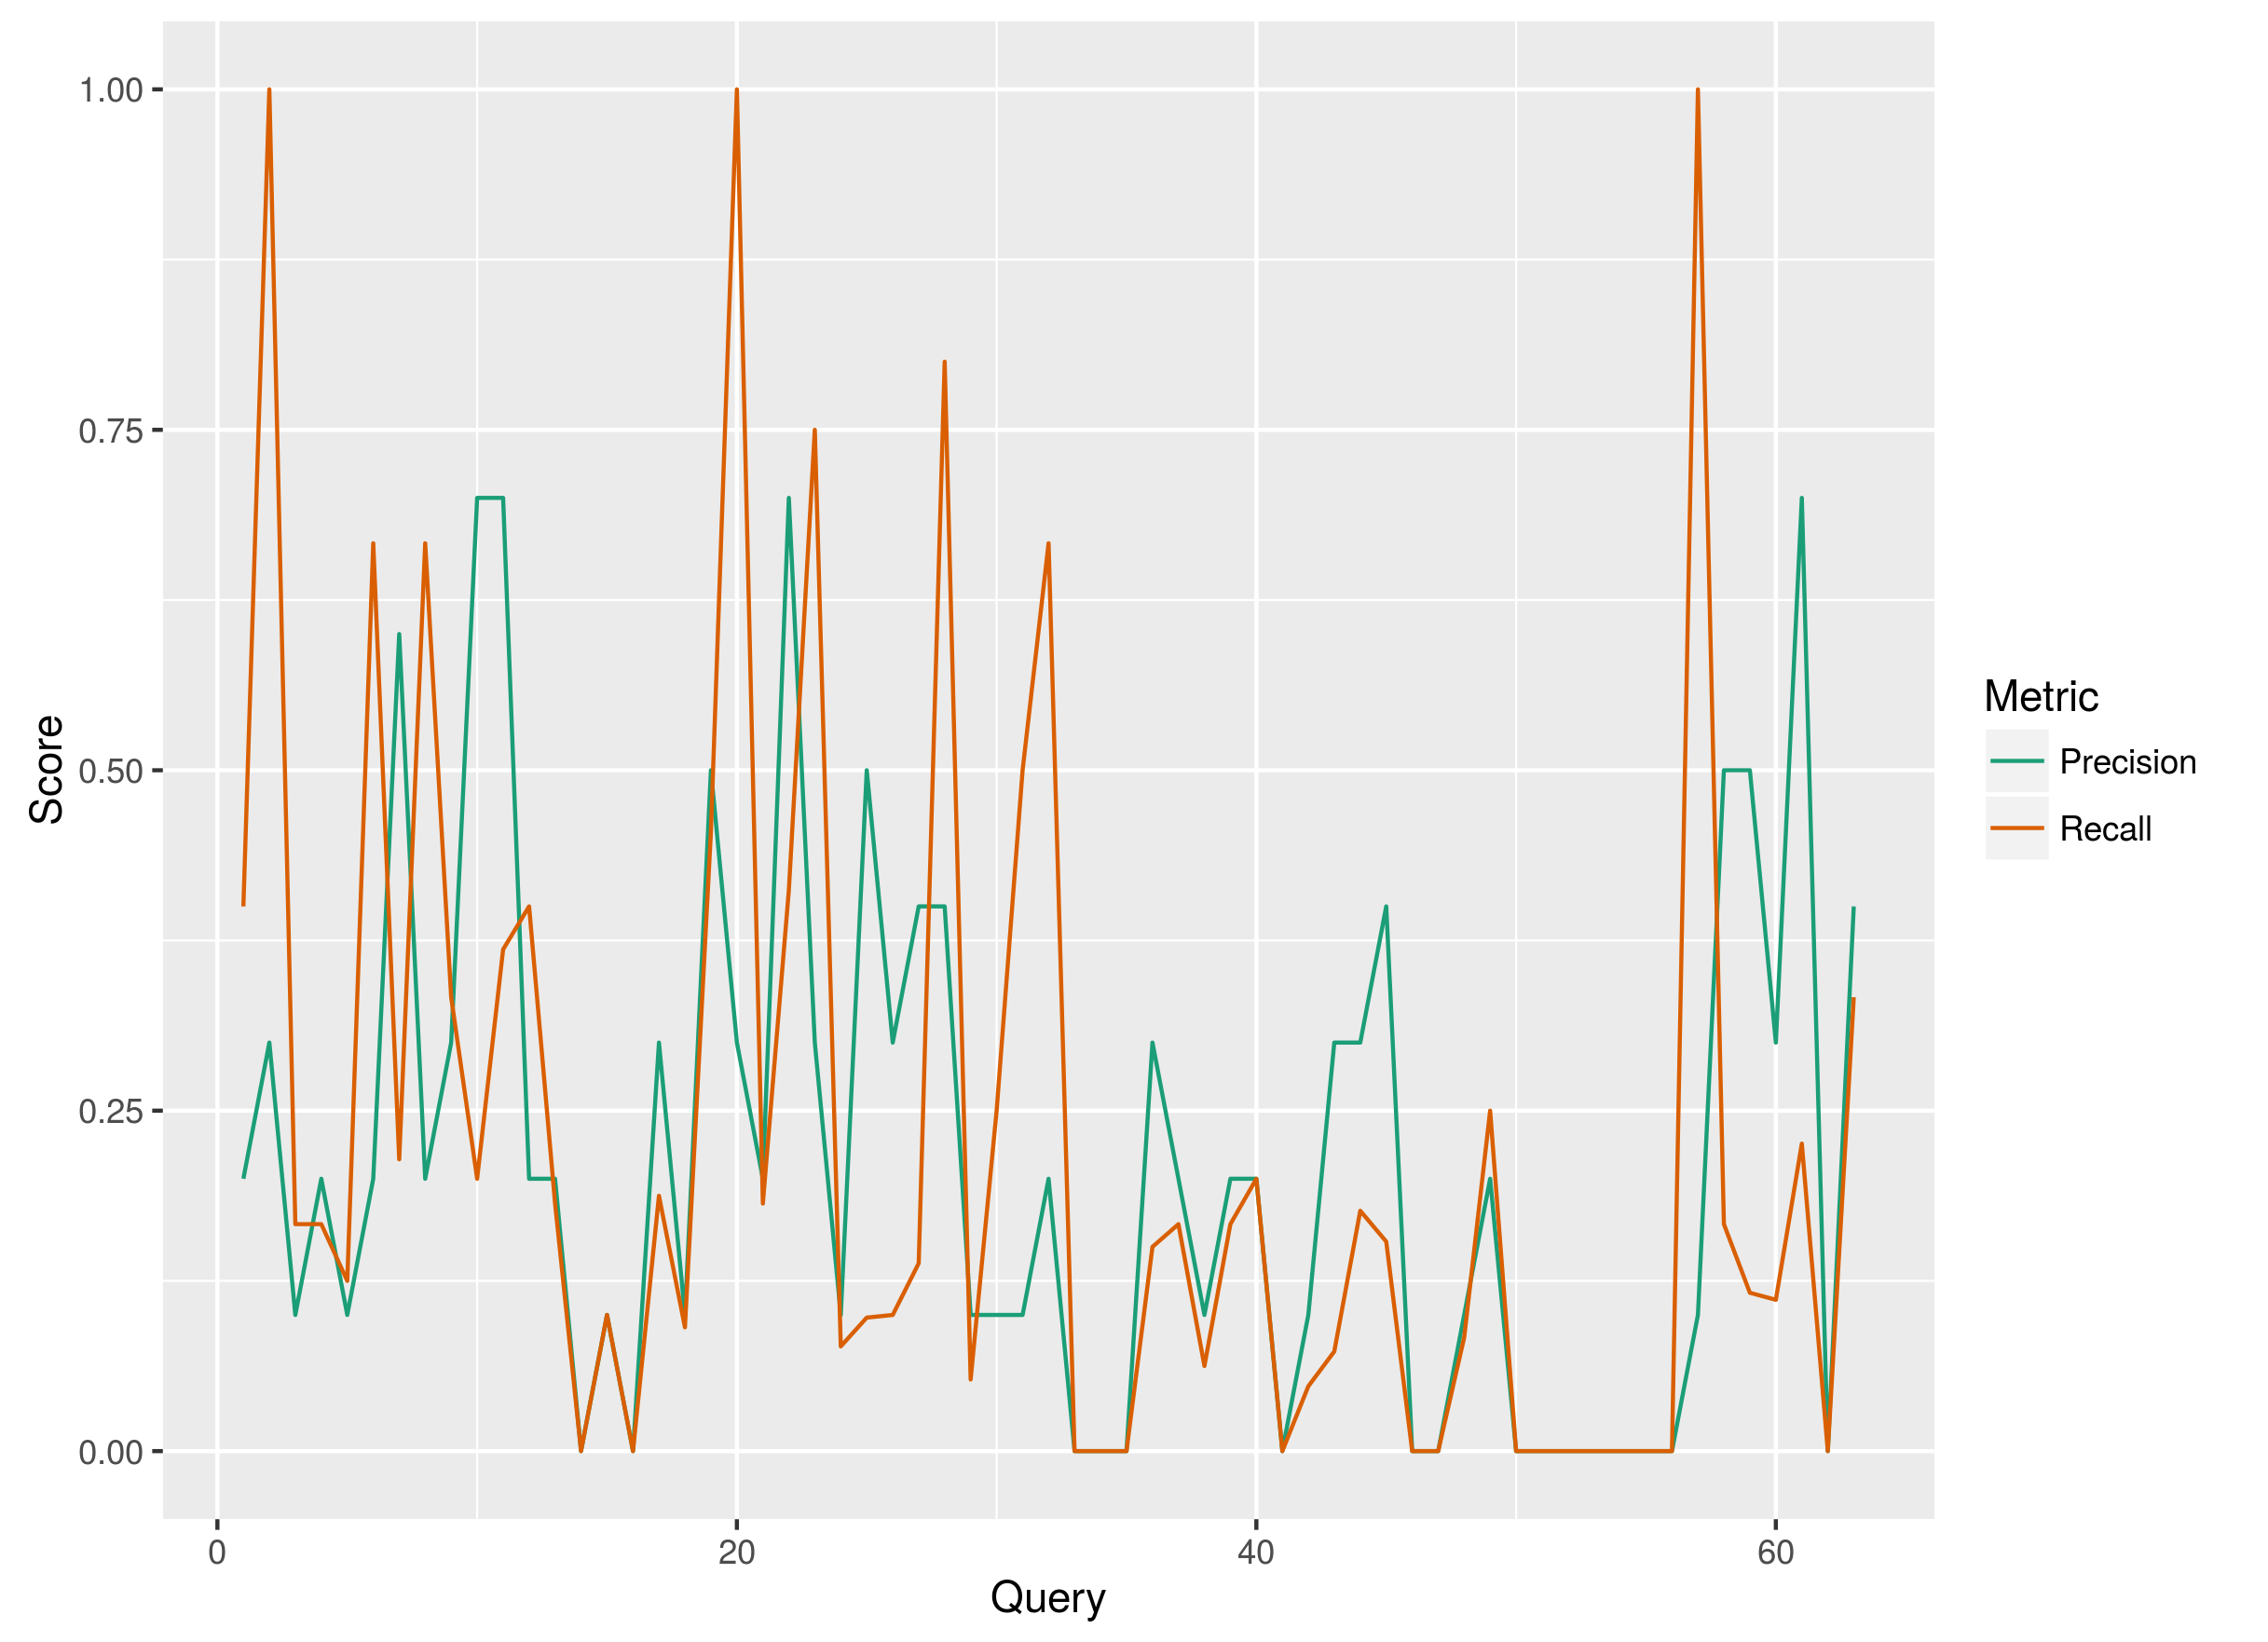
\includegraphics[scale=0.9]{q2_plot_rp.png}
\caption{Galago Eval Recall Precision For All Queries}
\label{fig:q2plot2}
\end{figure}
The seemingly eradicate hills and valleys are present in both plots and when considering \autoref{fig:q2plot2} it becomes clear that the overall performance of the queries was poor due to the number of queries with NaN values which were replaces with 0.0 in order to be included in these graphs.  Now consider \autoref{fig:q2plot3} which shows the number of relevant documents for the CACM queries it clearly shows the reason behind the result. 19 queries have less than 10 relevant queries.
\begin{table}[ht]
\centering
\caption{Relevant Document $<$ 10 Count }
\begin{tabular}{rr}
  \hline
 Query & Count \\ 
  \hline
 1 &   5 \\ 
2 &   3 \\ 
  3 &   6 \\ 
  5 &   8 \\ 
   6 &   3 \\ 
   8 &   3 \\ 
  9 &   9 \\ 
  12 &   5 \\ 
20 &   3 \\ 
   \hline
\end{tabular}
\end{table}
\begin{table}[ht]
\centering
\caption{Relevant Document $<$ 10 Count }
\begin{tabular}{rr}
  \hline
 Query & Count \\ 
  \hline
23 &   4 \\ 
  28 &   5 \\ 
   30 &   4 \\ 
31 &   2 \\ 
  32 &   3 \\ 
  33 &   1 \\ 
  49 &   8 \\ 
  57 &   1 \\ 
   62 &   8 \\ 
  64 &   1 \\ 
   \hline
\end{tabular}
\end{table}

\begin{figure}[H]
\centering
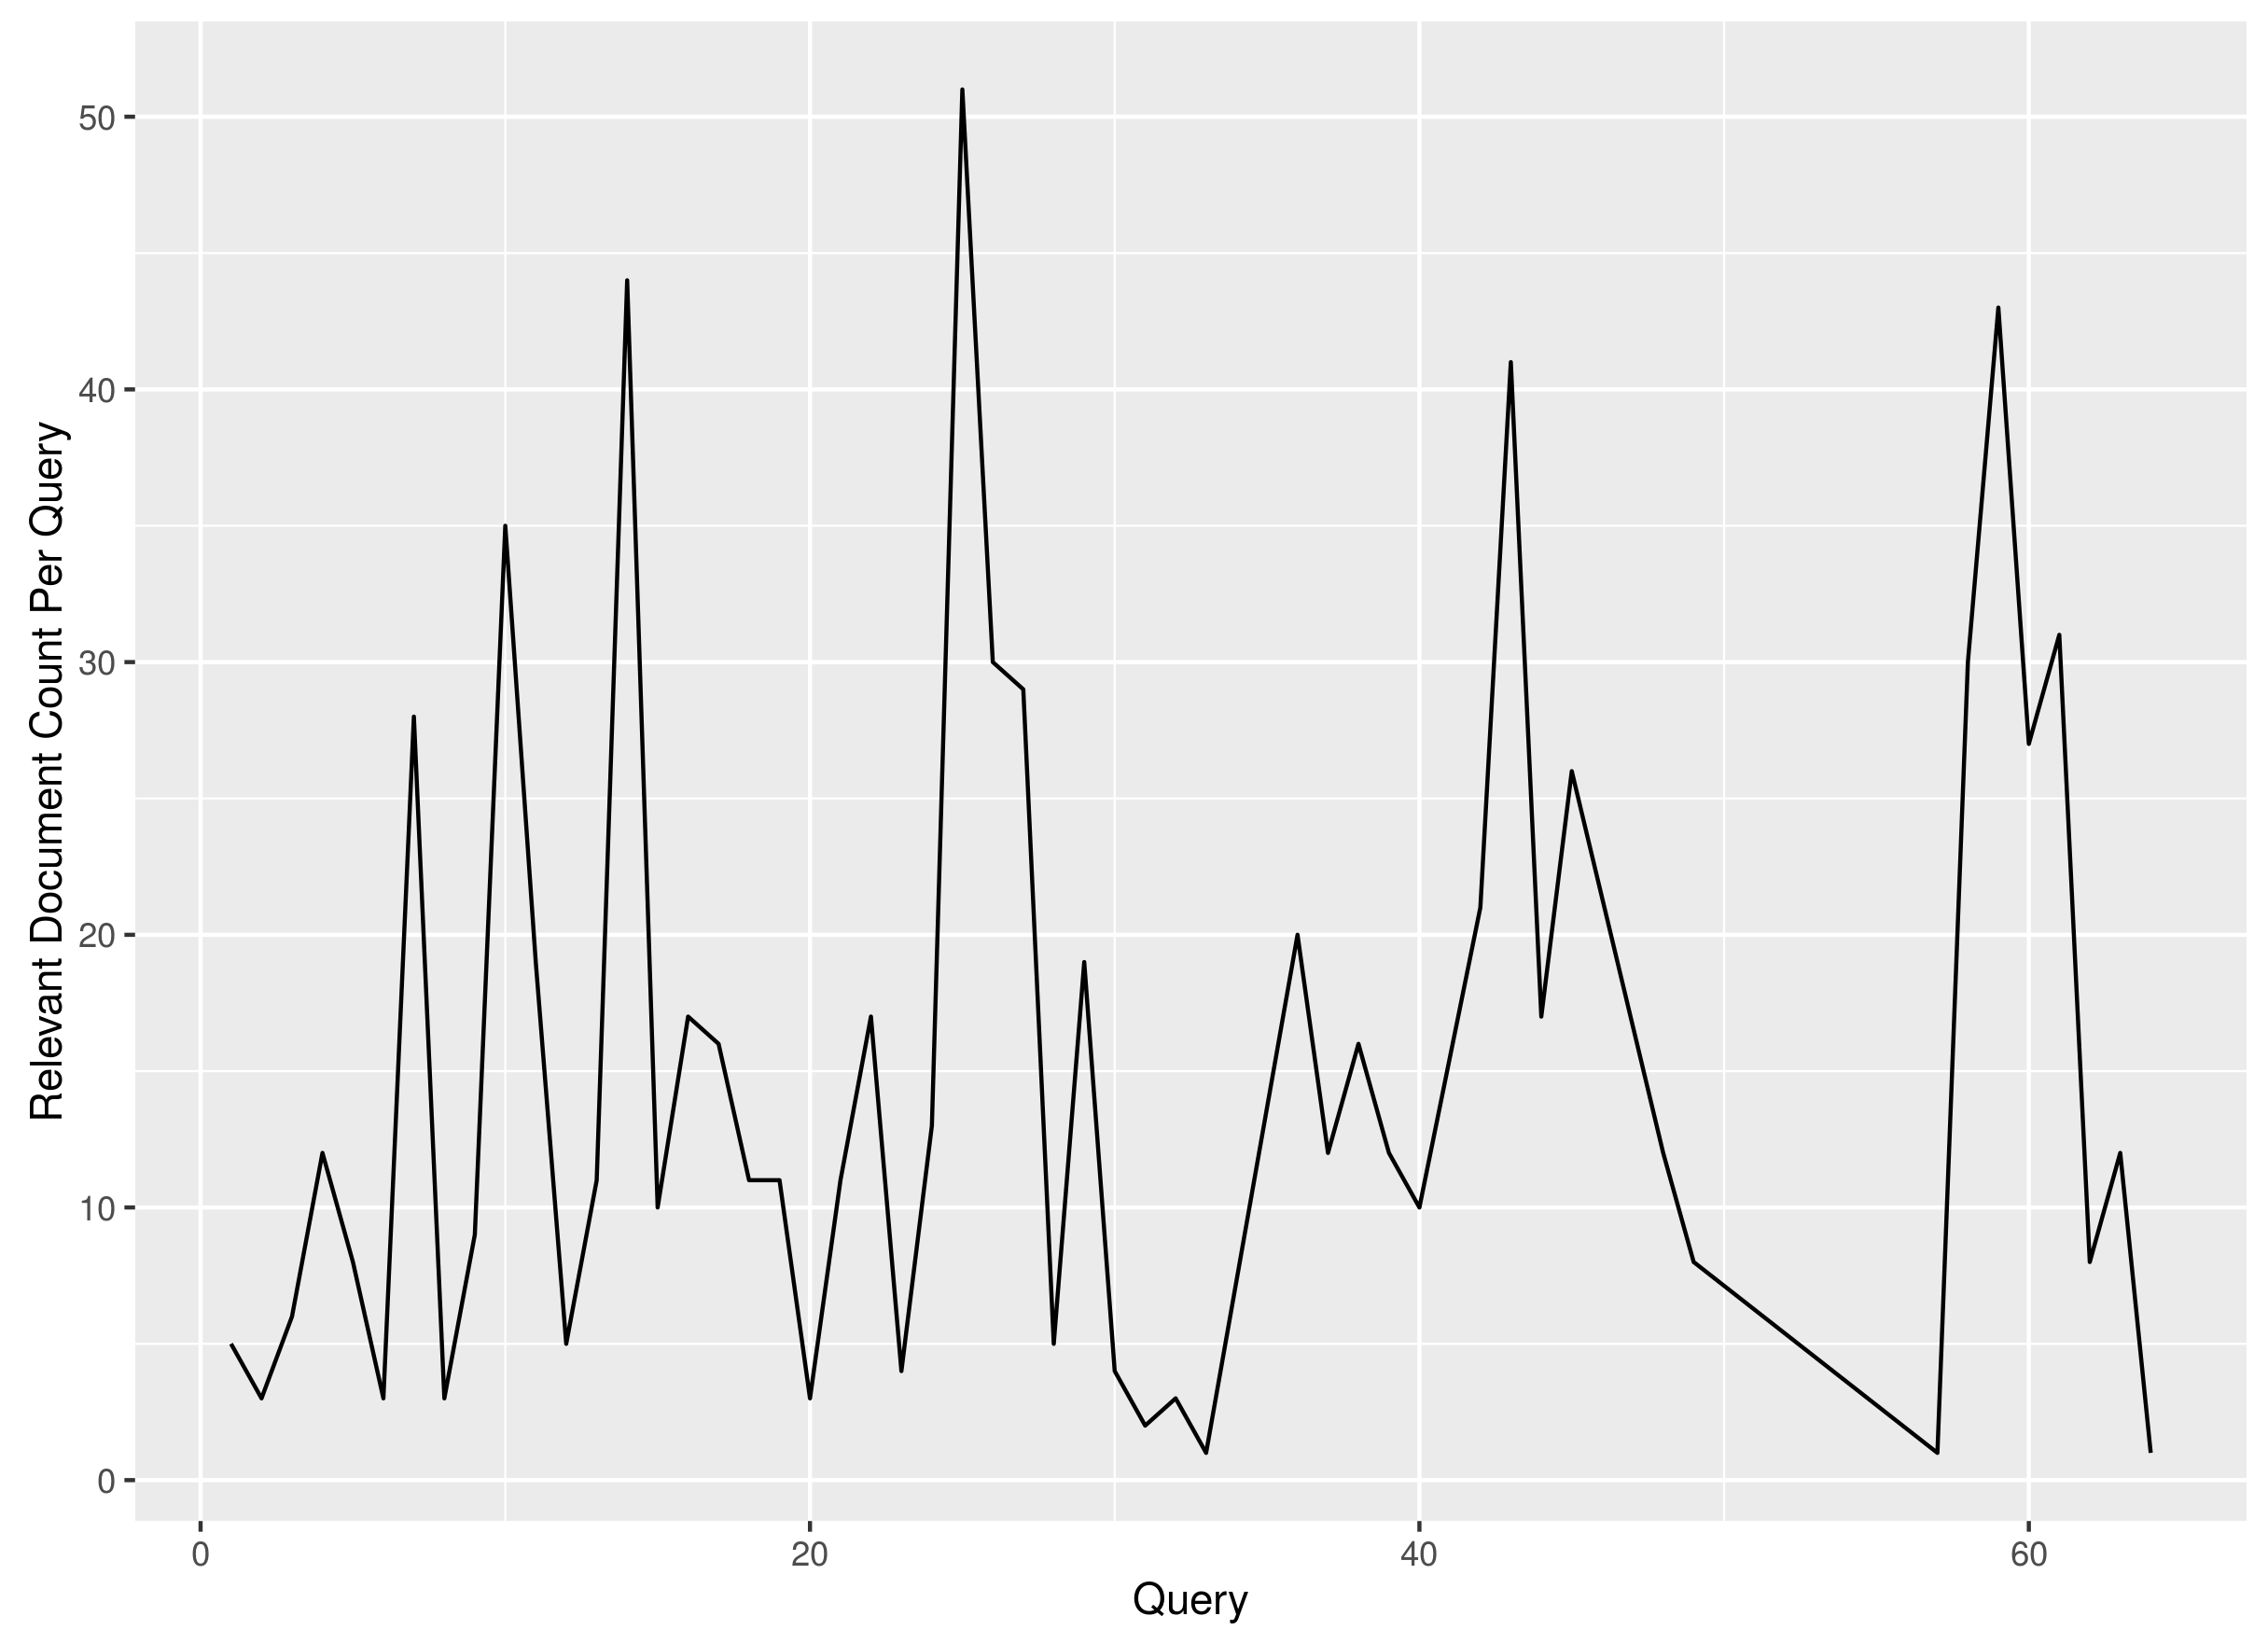
\includegraphics[scale=0.9]{q2_plot_rc.png}
\caption{Relevant Document Count For CACM Queries}
\label{fig:q2plot3}
\end{figure}
\begin{code}
\captionof{listing}{Graph Data File Generator} 
\label{code:q2py}
	\pycode{code/q2_8.5.py}
\end{code}
\begin{code}
\captionof{listing}{Graph Data File Generator Plotter} 
\label{code:q2r}
	\rcode{code/q2_plotter.R}
\end{code}
\begin{code}
\captionof{listing}{Ranking methods found on gist} 
\label{code:q1rnk}
	\pycode{code/ranking_methods.py}
\end{code}
\newpage
\begin{code}
\captionof{listing}{Context Helper Classes} 
\label{code:cntx}
	\pycode{code/contextClasses.py}
\end{code}
\newpage
\begin{code}
\captionof{listing}{CACM Helper Functions} 
\label{code:cacm_help}
	\pycode{code/cam_q_utils.py}
\end{code}

\begin{code}
\captionof{listing}{General Utility Functions} 
\label{code:util}
	\pycode{code/util.py}
\end{code}
\begin{code}
\captionof{listing}{Run Galago Bash File} 
\label{code:rungal}
	\shellcode{rungalago.sh}
\end{code}
\end{document}